\chapter{Tests and Results}
\label{tests}

In this chapter, several experiments will be performed in order to assess the quality and features of technologies and developed application. The main goals are: to obtain an empiric and realistic conclusion on which technology serves better the purpose of this thesis and to assess how the application fares when subject to different stress tests.

This chapter will be divided in two different sections: one regarding the comparison between Bluetooth and Wi-Fi Direct via different tests and other regarding the tests performed with the developed application, to better understand where it performs better and worse, proving or not if the theoretical choices made translate into actual performance gains.

\section{Bluetooth vs. Wi-Fi Direct}

This section will cover the differences, advantages and disadvantages of both Bluetooth and Wi-Fi Direct. A series of experiments will be conducted and their results analysed, providing a justification on which technology is best suited for this application and applications with a similar architecture and/or purpose.

Since the first implementation of Bluetooth in Android, several releases have been developed. Different Bluetooth versions provide different \gls{QoS}, this may impact the performed tests, as a device running a newer Bluetooth version may provide better results than a device running an older version. To avoid confusion, all the tested devices will be running Bluetooth version 4.0.

The tests will range from battery consumptions to data rates analysis, and most of the tests will be backed up by both theoretical and empirical results, although in some cases, due to the inability of getting precise measures, the results will be taken from previously developed works.

\subsection{Ranges of Communication}

The ranges of communication of both technologies are of extreme importance. They can reduce or increase greatly the number of hops a packet has to pass through, in order to reach the destination. If the range of communication is too short, the number of connections made will increase, this may cause an overload of the network, and the deterioration of the communication medium. On the other hand, if the communication range is long, the devices are able to jump through bigger hops, creating less traffic in the network and establishing the least possible number of connections.

Both technologies share some similarities: they depend on the environment of the communication, \textit{i.e.}, the elements that are surrounding the devices and possible obstacles in the way. The experiments were conducted, for the obstacle experiment, in a corridor of Torre Norte in the vicinities of Instituto Superior Técnico and, for the line of sight experiment in the outside area of Instituto Superior Técnico. It is important to note that although this experiments were made with as little interference as possible, there are certain elements that are impossible to controls, such as wireless communications from other devices and metal objects, such as metal lockers and cars.

Bluetooth establishes four different classes for the devices that may use this technology, depending on the transmitting power. Mobile phones are inserted in class 2 and, for that class, the specified average range of transmission in order to have a reliable connection is 10 meters, from \cite{bluetooth}.

Wi-Fi Direct on the other hand offers, theoretically, ranges of communication up to, approximately, 200 meters, from \cite{wfdrange}, which poses for a much better solution, in terms of network off-loading and general depth.

In order to verify these claims from both technologies, two mobile devices were taken to an open space, although with some limitations as described above, and several searches were made, until the devices stopped being discovered by one another. After measuring the distance between both devices, the results were taken, and prove what was already to be expected, although with some twists. 

Bluetooth was able to create a connection between devices from a distance up to 42 meters apart, see Figure \ref{fig:btMaxVisib} for the overall scheme of this experiment. This value is a lot more than what was expected judging by the theoretical value of 10 meters, although the health of the connection was not verified, see \ref{subsec:ftdr} for these tests. Using Wi-Fi Direct the devices were able to communicate from a maximum distance of 77 meters, see Figure \ref{fig:wfdMaxVisib} for the overall scheme of this experiment, which is, considerably, smaller than the theoretical value of 200 meters.

\begin{figure}[ht]
   \noindent\makebox[\textwidth]
    {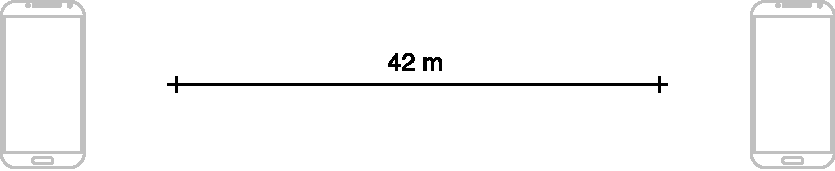
\includegraphics[width=0.8\textwidth]{images/bt_max_visib.pdf}}
	\caption{\label{fig:btMaxVisib} Max range of Bluetooth communication with line of sight between devices}
\end{figure}

\begin{figure}[ht]
   \noindent\makebox[\textwidth]
    {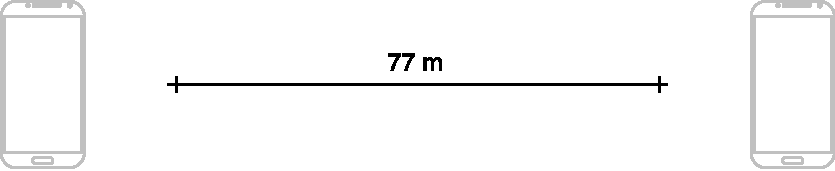
\includegraphics[width=0.8\textwidth]{images/wfd_max_visib.pdf}}
	\caption{\label{fig:wfdMaxVisib} Max range of Wi-Fi Direct communication with line of sight between devices}
\end{figure}

Both tests were made with a direct line of sight between devices. For the next ones there will be obstacles in the way of communication. It is expected that this affects greatly the communication ranges. The first test was made using Bluetooth technology where a wall was blocking the line of sight between devices, see Figure \ref{fig:btMaxInv}. The second test was made using Wi-Fi Direct, and, in order to maintain the same environment as the previous experiment, to get reliable results, it was situated in the same place as the first, see Figure \ref{fig:wfdMaxInv}. However, due to the environment configuration, it was impossible to recreate the experiment with only one wall, so two walls are now dividing the devices. Since the walls introduce a loss in the signal power, the more walls are between devices, the bigger the losses will be.

\begin{figure}[ht]
   \noindent\makebox[\textwidth]
    {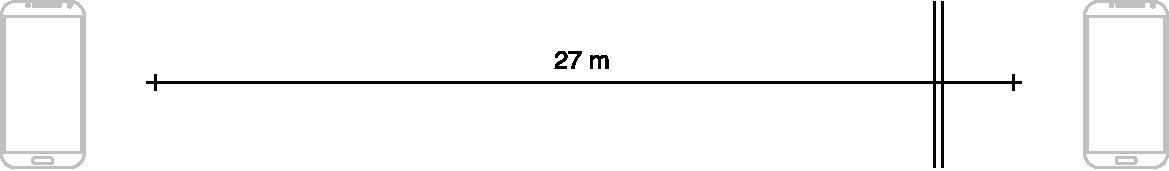
\includegraphics[width=0.8\textwidth]{images/bt_max_inv.pdf}}
	\caption{\label{fig:btMaxInv} Max range of Bluetooth communication without line of sight between devices}
\end{figure}

\begin{figure}[ht]
   \noindent\makebox[\textwidth]
    {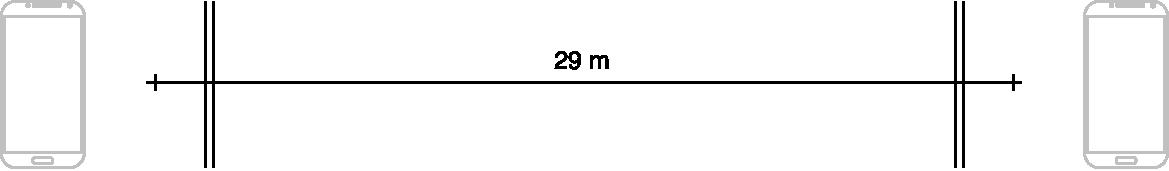
\includegraphics[width=0.8\textwidth]{images/wfd_max_inv.pdf}}
	\caption{\label{fig:wfdMaxInv} Max range of Wi-Fi Direct communication without line of sight between devices}
\end{figure}

As expected the obstacle, in this case the wall, created a significant decrease on the maximum range of communication. Bluetooth was able to communicate from a distance of 27m, closer to the theoretical 10 meters.

Wi-Fi Direct was also able to communicate from a smaller maximum distance, measuring 29 meters with the signal passing through both walls. From a smaller distance, it was verified that this technology could communicate with only wall in the way, meaning it also surpasses Bluetooth when an obstacle is in the way of communication.

After these experiments, it is possible to conclude that Wi-Fi Direct is more desirable, since it provides better coverage than Bluetooth to similar areas. Also, there is no evidence that Wi-Fi Direct suffers more losses from obstacles, maintaining its desirability. This was already to expect, both from the theoretical values and from the transmission powers\footnote{Transmission powers impact directly the range of transmission, since they affect the signal strength, a crucial characteristic for receivers to better capture the transmissions. A bigger transmit power, usually, creates a bigger signal strength leading to the signal being capture over bigger distances, as referred in \cite{txpower}, for instance.}, since Bluetooth is mostly known for its lower transmit powers, if compared to Wi-Fi.

\subsection{Battery Consumptions}

\subsection{Discovery Times}
\label{subsec:normaldisc}

The discovery time is a critical factor for this work. The discovery process is one of the biggest time consumers during an application run. Thus, minimizing it, is a great advantage for the overall performance of the application.

For the purpose of testing the Bluetooth and Wi-Fi Direct discovery times, three mobile devices were used: Samsung Grand Neo, running Android version 4.2.2; Motorola Moto G2, running Android version 7.1; Huawei P8 Lite, running Android version 6.0, providing an heterogeneous sample space.

Every device is running Bluetooth version 4.0. This Bluetooth version theoretically provides a discovery time of 10.24s, as mentioned in \cite{btdisc1} and \cite{btdisc2}. To confirm this hypothesis, discovery times values from the three devices were measured. Each device was submitted to multiple discoveries with a different number of discovered peers, ranging from 0 to 3 peer devices found.

Figure \ref{fig:normaldisc} shows the measured Bluetooth discovery times from the three tested devices. It is important to note that these results were measured with a chronometer, having a maximum precision of 0.5s.

Samsung Grand Neo (in blue) is constant throughout the measuring, having a Bluetooth discovery time of 13s. Motorola Moto G2 (in green) shows some variance in the various measurements. The Bluetooth discovery time measures range from 13s to 14s, having an average of 13.85s. Huawei P8 Lite (in purple) shows the biggest deviation throughout the sample space. Its Bluetooth discovery time measures range from 16.5s to 15s, having an average of 15.976s.

\begin{figure}[ht]
	\noindent\makebox[\textwidth]
	{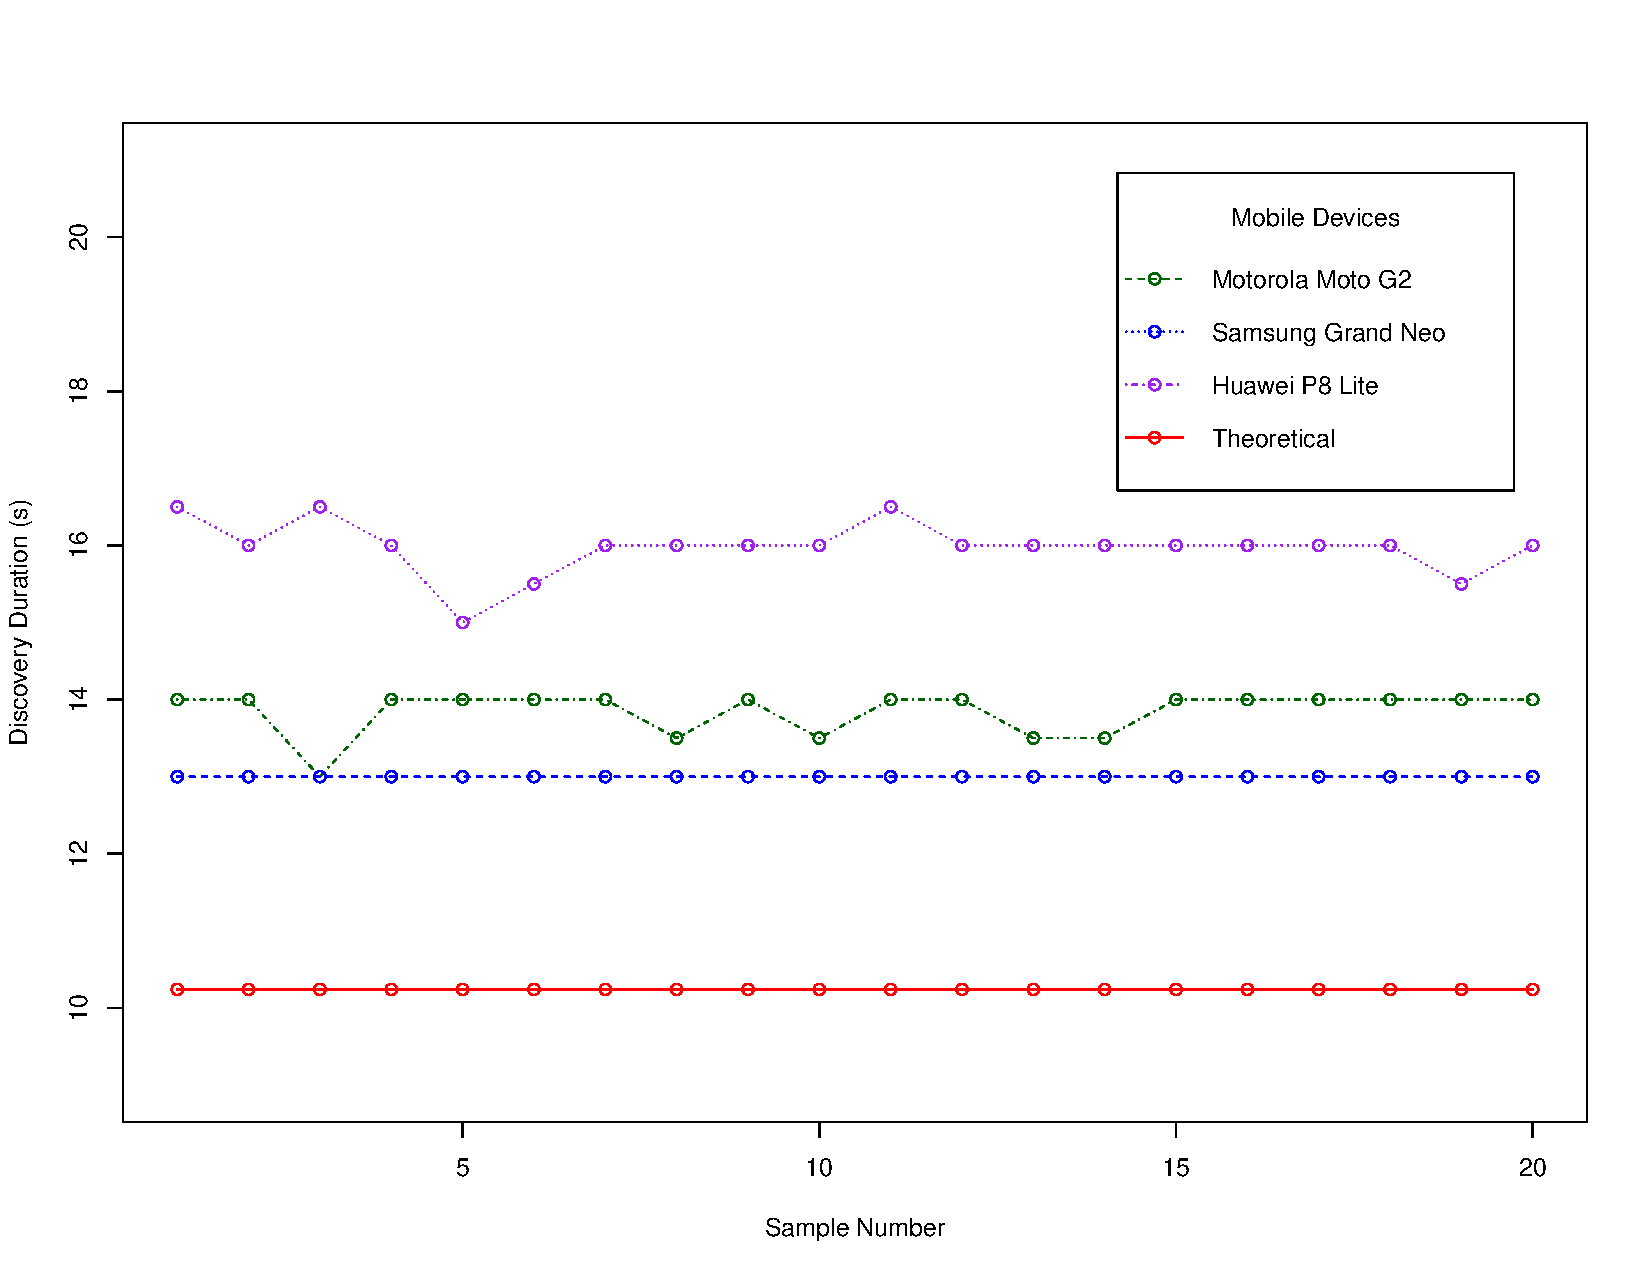
\includegraphics[width=1\textwidth]{images/plot_normal_disc.pdf}}
	\caption{\label{fig:normaldisc} Plot of the measured Bluetooth discovery times from the three devices.}
\end{figure}

None of the three devices approached the theoretical Bluetooth discovery time value of 10.24s, the difference is quite significant in a delay-sensitive application, such as the developed one.

Each device showed a different average Bluetooth discovery time, this difference in the discovery times can be due to the different hardware used in the devices, since each device is produced by a different manufacturer.

\subsection{File Transfer Data Rates}
\label{subsec:normalftdr}

\section{Testing the Developed Application}

In this section several tests will be executed, aiming to provide an overview of the developed application's performance. A conclusion will be given, reflecting on where the application performs the best and worse.

\subsection{Discovery Times}
\label{subsec:appdisc}

In this subsection the developed application discovery times will be tested. To obtain a meaningful analysis, the devices used are the same as the ones used in Subsection \ref{subsec:normaldisc}. It is expected that the measured discovery time values don't differ greatly from the ones previously obtained in Subsection \ref{subsec:normaldisc}.

Once again, the discovery times are measured in the same conditions as in Subsection \ref{subsec:normaldisc} and the number of discovered peer devices ranges from 0 to 2 devices found. However, to retrieve the Bluetooth discovery times the Android debugger was used, providing a precision of 0.5ms.

In Figure \ref{fig:appdisc}, the times measured during the developed application's discovery are shown, alongside the theoretical value of 10.24s, mentioned in Subsection \ref{subsec:normaldisc}.

Analysing the plot it is possible to see that (1) Samsung Grand Neo (in blue) shows the best Bluetooth discovery times, being almost constant throughout the sample space. It provides an average discovery time of 12.826s; (2) Motorola Moto G2's (in green) discovery times were similar to Samsung Grand Neo's discovery times, except for punctual samples, where the times are slightly bigger. It provides an average discovery time of 12.991s; (3) Huawei P8 Lite (in purple) provides the most irregular measures, similarly to what happened in Subsection \ref{subsec:normaldisc}. Its measured times range from 15 to 18s, having an average of 16.755s.

\begin{figure}[ht]
	\noindent\makebox[\textwidth]
	{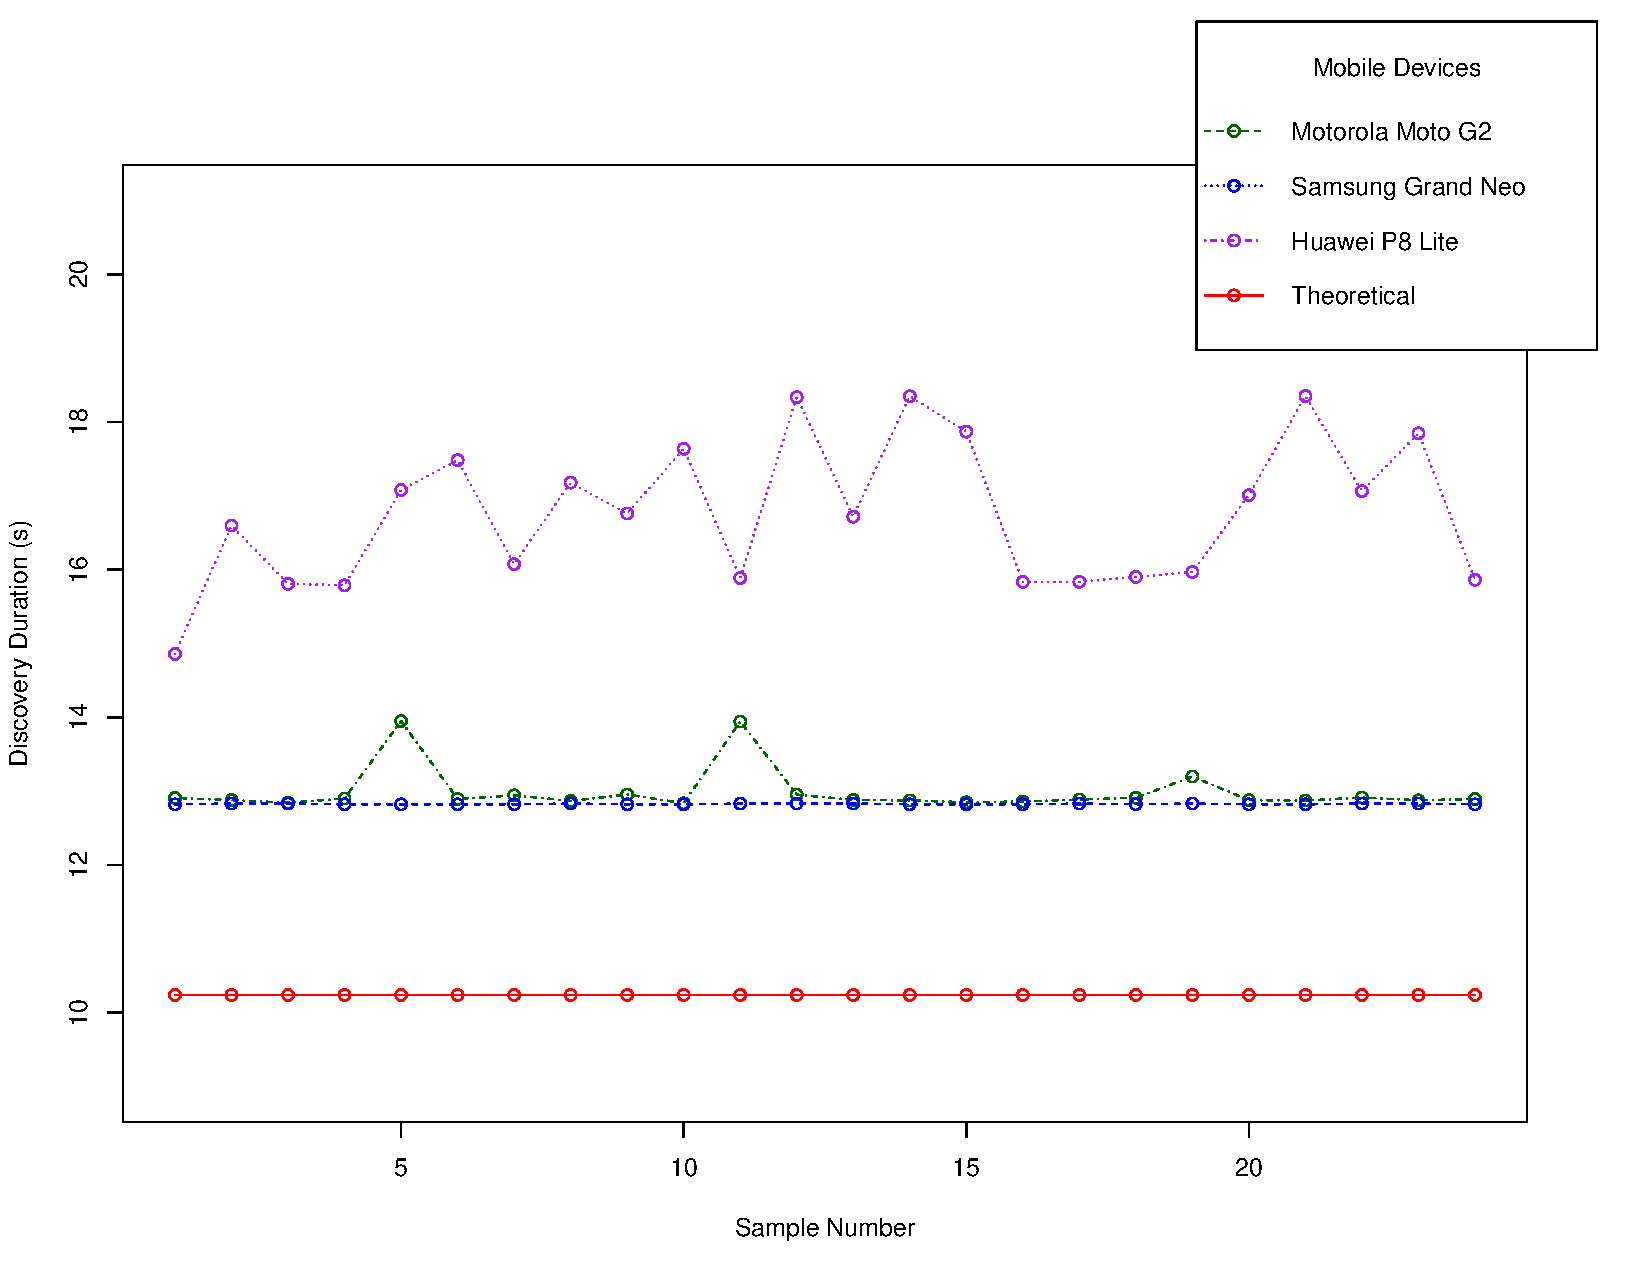
\includegraphics[width=1\textwidth]{images/plot_app_disc.pdf}}
	\caption{\label{fig:appdisc} Plot of the Bluetooth discovery times measured while using the developed application from the three devices.}
\end{figure}

As expected, the measured application discovery times were very similar to the ones obtained during a native discovery time. All the devices maintained the same properties they presented in \ref{subsec:normaldisc}: Samsung Grand Neo was mostly constant in both tests, providing the lowest discovery times; Motorola Moto G2 provided the second best discovery times, showing less deviation from the average in the current test than during the test performed in \ref{subsec:normaldisc}; Huawei P8 Lite showed the worst discovery times, however its average discovery time was similar in both tests. It also showed the most deviation from the average in both tests, having a bigger amplitude of results in the current test, as mentioned before.

Once again, it is possible to see that all three devices failed to meet the theoretical value of 10.24s, having shown discovery time averages of the theoretical time plus 2 to 4s.

\subsection{Advertisement Times}

\subsection{File Transfer Data Rates}

\subsection{Battery Consumption During Use}




